                %!TEX program = xelatex
\documentclass[9pt, compress]{beamer}
\usetheme[sectionpage=progressbar]{metropolis}

\usepackage{booktabs}  
\usepackage[scale=2]{ccicons}
\usepackage[T1]{fontenc}
\usepackage[utf8]{inputenc}
\usepackage{lmodern}
\usepackage{amsthm}
\usepackage{diagbox} %tabelas com barras
\usepackage{booktabs}
\usepackage{graphicx}			% Inclusão de gráficos

\author{\textbf{Matheus S. D'Andrea Alves}, \textbf{Uéverton dos Santos Souza} } 
\title{Parametrized Complexity on the Graph(r,l) class}
\subtitle{Minimum vertex coloring on Graphs(r,l)}
%\logo{}
\institute{\textbf{Universidade Federal Fluminense}}
\date{Ocotber 2017}
%\subject{}
%\setbeamercovered{transparent}
%\setbeamertemplate{navigation symbols}{}
\begin{document}
    \maketitle
    \begin{frame}{Overral}
    \centering
        \tableofcontents
    \end{frame}
    \section{Introduction}
    \begin{frame}
        \frametitle{Who am I}
        \begin{columns}
          \begin{column}{0.3\textwidth}
            \includegraphics[scale=0.2]{../figuras/foto.jpg}
          \end{column}
          \begin{column}{0.5\textwidth}
            Undergraduated student at:
            \begin{itemize}
              \item Universidade Federal Fluminense
            \end{itemize}
            
            Interested in:
            \begin{itemize}
              \item Graph theory
              \item Complexity analysis
              \item Software engineering
            \end{itemize}
            
            You can find me here:
            \begin{itemize}
              \item \url{github.com/MSDandrea}
              \item \url{telegram.me/MSDandrea}
            \end{itemize}
          \end{column}
        \end{columns}
    \end{frame}
    \section{The problem}
    \begin{frame}{Basic concepts}
      \begin{columns}
        \begin{column}{0.5\textwidth}
          \textbf{Graph(r,l)}
          
          Any graph in the class of graphs that can be partitionated in $r$ independent sets and $l$ cliques
        \end{column}
        \begin{column}{0.5\textwidth}
          \textbf{Minimum vertex coloring}
          
          A minimum vertex coloring is an assignment of a color among $k$ colors to each vertex of a graph such that no edge connects two identically colored vertices and $k$ is the smallest value to obtain a k-coloring
        \end{column}
      \end{columns}
    \end{frame}
    \begin{frame}[standout]
      THE QUESTION:
      
      When does this problem begins to be NP-Complete? 
      
      And why?
    \end{frame}
    \section{Our approach}
    \begin{frame}{The idea}
      Build a dichotomy to the problem, based on the $r$ and $l$ values.
      
      Gather the results and search for a pattern in the problem behavior.
    \end{frame}
    \begin{frame}{First steps}
      The starting point was the following:
      \begin{itemize}
        \item A null Graph (i.e. a Graph(0,0)) is 0-colorable.
        \item 
        \item 
        \item 
         \item                                                                                                                
      \end{itemize}
    \end{frame}
    \begin{frame}{First steps}
      The starting point was the following:
      \begin{itemize}
        \item A null Graph (i.e. a Graph(0,0)) is 0-colorable.
        \item A empty Graph (i.e. a Graph(1,0)) is 1-colorable.
        \item 
        \item 
         \item                                                                                                                
      \end{itemize}
    \end{frame}
    \begin{frame}{First steps}
      The starting point was the following:
      \begin{itemize}
        \item A null Graph (i.e. a Graph(0,0)) is 0-colorable.
        \item A empty Graph (i.e. a Graph(1,0)) is 1-colorable.
        \item A bipartide Graph (i.e. a Graph(2,0)) is 2-colorable.
        \item 
         \item                                                                                                                
      \end{itemize}
    \end{frame}
    \begin{frame}{First steps}
      The starting point was the following:
      \begin{itemize}
        \item A null Graph (i.e. a Graph(0,0)) is 0-colorable.
        \item A empty Graph (i.e. a Graph(1,0)) is 1-colorable.
        \item A bipartide Graph (i.e. a Graph(2,0)) is 2-colorable.
        \item A Complete Graph (i.e. a Graph(0,1)) is k-colorable where $k = \#V(G)$.
        \item                                                                                                               
      \end{itemize}
    \end{frame}
    \begin{frame}{First steps}
      The starting point was the following:
      \begin{itemize}
        \item A null Graph (i.e. a Graph(0,0)) is 0-colorable.
        \item A empty Graph (i.e. a Graph(1,0)) is 1-colorable.
        \item A bipartide Graph (i.e. a Graph(2,0)) is 2-colorable.
        \item A Complete Graph (i.e. a Graph(0,1)) is k-colorable where $k = \#V(G)$.
        \item A Split Graph (i.e. a Graph(1,1)) is k-colorable where $k = \#V(C)$ such that C is the Maximal clique in G.
      \end{itemize}
    \end{frame}
    \begin{frame}{Further}
      \begin{theorem}
        Minimum vertex coloring of Graph(0,2) is Polynomial.
     \end{theorem}
     \begin{proof}
      A Graph(0,2) is a Graph that can be partiotionated into 2 cliques, finding the maximal clique in this case is polynomial. 
      Once we have the maximal clique, we known that the graph can be colored with k colors, such that K is the maximal clique cardinality.
     \end{proof}
    \end{frame}
    \begin{frame}{Further}
      \begin{theorem}
        Minimum vertex coloring of Graph(3,0) is Polynomial.
     \end{theorem}
     \begin{proof}
      Beacause we know that the Graph is a Graph(3,0) we known it can be colored at most with 3 colors.
      To find out if it can be colored with 2 or one color is polynomial, implying that minimum vertex coloring of Graph(3,0) is Polynomial.
     \end{proof}
    \end{frame}
    \begin{frame}{Further}
      \begin{theorem}
        Minimum vertex coloring of Graph(4,0) is NP-Complete.
     \end{theorem}
     \begin{proof}
      We know that the Graph is a Graph(4,0), therefore it can be colored at most with 4 colors.
      We need to discover if it can be colored with 3 colors; 
      Note that if the graph is a planar graph then 3-coloring is NP-Complete, therefore minimum vertex coloring of Graph(4,0) is NP-Complete.
     \end{proof}
    \end{frame}
    \section{First results}
    \begin{frame}{Partial Dichotomy}
        \begin{table}[htb!]
          \center
          \begin{tabular}{l|*{7}c}
            \toprule
            \backslashbox{$r$}{$l$} & 0 & 1 & 2 & 3 & 4 & \ldots & n\\
            \midrule
            0 & \textit{P} & \textit{P} & \textit{P} & ? & ? & \ldots & ?\\
            1 & \textit{P} & \textit{P} & ? & ? & ? & \ldots & ?\\
            2 & \textit{P} & ? & ? & ? & ? & \ldots & ?\\
            3 & \textit{P} & ? & ? & ? & ? & \ldots & ?\\
            4 & \textit{NPc} & \textit{NPc} & \textit{NPc} & \textit{NPc} & \textit{NPc} & \ldots & \textit{NPc}\\
            $\vdots$ & $\vdots$ & $\vdots$ & $\vdots$ & $\vdots$ & $\vdots$ & $\ddots$ & \textit{NPc}\\
            n & \textit{NPc} & \textit{NPc} & \textit{NPc} & \textit{NPc} & \textit{NPc} & \ldots & \textit{NPc}\\
            \bottomrule
          \end{tabular}%
          \caption{Partial dichotomy of the minimum vertex coloring problem on Graph(r,l)}
          \label{tab:tabela_part2dictrl}%
        \end{table}%
    \end{frame}
    \begin{frame}[standout]
      How to proceed?
    \end{frame}
    \section{The relation between list coloring and minimum vertex coloring in Graph(r,l)}
    \begin{frame}{The relation between list coloring and minimum vertex coloring in Graph(r,l)}
        \begin{theorem}
          Minimum vertex coloring is NP-Complete for Graph(r,l+1) if list coloring is NP-Complete for Graph(r,l)
        \end{theorem}
    \end{frame}
    \begin{frame}{The relation between list coloring and minimum vertex coloring in Graph(r,l)}
        \textbf{Proof.}
        
        The proof consists in showing that a solution for the list coloring problem in a Graph(r,l) G, implies in a solution for the minimum color problem in a Graph(r,l+1) $H_G$.
        
        In order to do so, we need to show that:
          \begin{itemize}
        \item If a graph G(r,l) has a proper list coloring then $H_G$ is k-colorable for k=total number of colors in the lists (1).
        \item If $H_G$ is k-colorable then G has a proper list coloring (2).
      \end{itemize}
    \end{frame}
    \begin{frame}{The relation between list coloring and minimum vertex coloring in Graph(r,l)}
      \textbf{(1):}
      
      Let G be a Graph(r,l) such that each vertex $v \in V(G)$ has a color list; 
      Each list has at least one color of the Set: $C = \{c_1,c_2,c_3,...,c_k \}$. 
      \begin{center}
        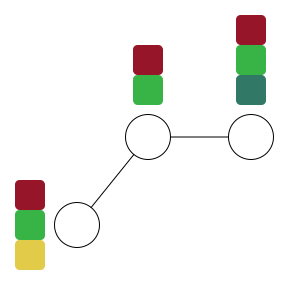
\includegraphics[scale=0.4]{../figuras/presentation-G.png}
      \end{center}
    \end{frame}
    \begin{frame}
      Let G be a \textbf{yes} instance for the list coloring problem, we build a clique K, where each vertex $u \in V(K)$ represents a color of C.
      \begin{center}
        \includegraphics[scale=0.4]{../figuras/presentation-K.png}
      \end{center}
      Note that the clique K has exactly k vertices, thereafter, we can colorize K with only k colors, without becoming restrictive whe can asume that the vertex $u_i \in K$ will be colored with the color $c_i$.
    \end{frame}
    \begin{frame}  
      Supose $H_G$ $= G \cup K$, and that for every vertex $u_i \in V(K)$ and every vertex $v_j \in V(G)$ add a edge $E(u_i,v_j) $ in $H_G$ iff $c_i$ is not a color present on the list of $v_j$.
      \begin{center}
        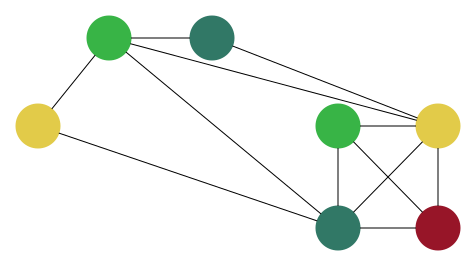
\includegraphics[scale=0.4]{../figuras/presentation-H.png}
      \end{center}   
      Using this construction, the coloring of K does not conflict with the color pattern solution found for G, implying in a minimum proper coloring of $H_G$. 
    \end{frame}
    \begin{frame}{The relation between list coloring and minimum vertex coloring in Graph(r,l)}
      \textbf{(2):}
      
      We know that the graph $H_G$ is a Graph(r,l+1) and has a k-coloring. Let K be the maximal clique in $H_G$.
      We also know that k is the number of vertices in K.
      
      Note that the removal of K from $H_G$ (which will become G) does not affect it's proper coloring, also note that for the remaining vertex $v \in V(G)$ we can now build a list of colors from their formers non-neighboors in K in such a way that it does not affect it's proper coloring.
      
      In that way we show that, if $H_G$ is k-colorable, G is a yes instance for the list coloring problem.
      $\qed$
    \end{frame}
    \begin{frame}{Corollaries}
      With this result we can say that:
      \begin{itemize}
        \item Minimum proper coloring of Graph(1,2) is NP-Complete.\newline NP-Completeness of list coloring of split graphs was demonstrated by Jensen et al. at \textit{"Generalized coloring for tree-like graphs"}.
        \item Minimum proper coloring of Graph(2,1) is NP-Complete\textbf{*}.\newline NP-Completeness of list coloring of bipartide graphs was demonstrated by Fellows et al. at \textit{"List Coloring and Precoloring Extension are W[1]-hard parameterized by treewidth"}.
        \item Minimum proper coloring of Graph(0,3) is NP-Complete.
        \newline NP-Completeness of list coloring of Graph(0,2) graphs was demonstrated by Jensen et al. at \textit{"Complexity results for the optimum cost chromatic partition problem"}.
      \end{itemize}
    \end{frame}
    \begin{frame}{ Peculiarity of Graphs(2,1) }
      It's trivial to see that the coloring problem for this specific class has a clear upper and lower bound (K+1 and K respectively), but beside the bounds it is still NP-Complete to determine which one it is.
    \end{frame}
    \section{Final results}
    \begin{frame}{On minimum coloring}
        These results allow us to finish our dichotomy.
        
        \begin{table}[htb!]
          \center
          \begin{tabular}{l|*{7}c}
            \toprule
            \backslashbox{$r$}{$l$} & 0 & 1 & 2 & 3 & 4 & \ldots & n\\
            \midrule
            0 & \textit{P} & \textit{P} & \textit{P} & \textit{NPc} & \textit{NPc} & \ldots & \textit{NPc}\\
            1 & \textit{P} & \textit{P} & \textit{NPc} & \textit{NPc} & \textit{NPc} & \ldots & \textit{NPc}\\
            2 & \textit{P} & \textit{NPc} & \textit{NPc} & \textit{NPc} & \textit{NPc} & \ldots & \textit{NPc}\\
            3 & \textit{P} & \textit{NPc} & \textit{NPc} & \textit{NPc} & \textit{NPc} & \ldots & \textit{NPc}\\
            4 & \textit{NPc} & \textit{NPc} & \textit{NPc} & \textit{NPc} & \textit{NPc} & \ldots & \textit{NPc}\\
            $\vdots$ & $\vdots$ & $\vdots$ & $\vdots$ & $\vdots$ & $\vdots$ & $\ddots$ & \textit{NPc}\\
            n & \textit{NPc} & \textit{NPc} & \textit{NPc} & \textit{NPc} & \textit{NPc} & \ldots & \textit{NPc}\\
            \bottomrule
          \end{tabular}%
          \caption{Dichotomy of the minimum vertex coloring problem on Graph(r,l)}
          \label{tab:tabela_dictrl}%
        \end{table}%
    \end{frame}
    \begin{frame}{On clique cover}
      Coloring of a Graph $G$ may be seen as \textit{Clique cover} of it's complement $G'$, impling in:
      
       \begin{table}[htb!]
          \center
          \begin{tabular}{l|*{7}c}
            \toprule
            \backslashbox{$r$}{$l$} & 0 & 1 & 2 & 3 & 4 & \ldots & n\\
            \midrule
            0 & \textit{P} & \textit{P} & \textit{P} & \textit{P} & \textit{NPc} & \ldots & \textit{NPc}\\
            1 & \textit{P} & \textit{P} & \textit{NPc} & \textit{NPc} & \textit{NPc} & \ldots & \textit{NPc}\\
            2 & \textit{P} & \textit{NPc} & \textit{NPc} & \textit{NPc} & \textit{NPc} & \ldots & \textit{NPc}\\
            3 & \textit{Npc} & \textit{NPc} & \textit{NPc} & \textit{NPc} & \textit{NPc} & \ldots & \textit{NPc}\\
            4 & \textit{NPc} & \textit{NPc} & \textit{NPc} & \textit{NPc} & \textit{NPc} & \ldots & \textit{NPc}\\
            $\vdots$ & $\vdots$ & $\vdots$ & $\vdots$ & $\vdots$ & $\vdots$ & $\ddots$ & \textit{NPc}\\
            n & \textit{NPc} & \textit{NPc} & \textit{NPc} & \textit{NPc} & \textit{NPc} & \ldots & \textit{NPc}\\
            \bottomrule
          \end{tabular}%
          \caption{Dichotomy of the clique cover problem on Graph(r,l)}
          \label{tab:tabela_dictrl}%
        \end{table}%
    \end{frame}
    \begin{frame}[standout]
      Does the Minimum vertex coloring problem has a parametrized solution for Graph(r,l)?
    \end{frame}
    \begin{frame}{Graph(2,1)}
      \large{Parametrized by the size of the smallest independent set}
      \normalsize\newline\newline
      We know the clique can be colored with k colors.
      
      We know that we can transform a minimun coloring problem into a list coloring problem.
      
      Fellows showed that the list coloring problem is w[1]-hard for bipartide graph when parametrized by the size of the smallest independent set.
      
      Minimal vertex coloring is w[1]-hard when parametrized by the smallest independet set in a Graph(2,1).
    \end{frame}
    \begin{frame}{Conclusion}
       We were sucessfull in building our foundation, answering our first question, and discovered a interesting relation between two coloring problems applied to the Graph(r,l) class.
       
       Future works:
       \begin{itemize}
         \item Why the problem behave that way?
         \item Does the Minimum vertex coloring problem has a parametrized solution for Graph(r,l)?
       \end{itemize}
     \end{frame}
     \begin{frame}[standout]
       THANK YOU!
       
       Questions?
     \end{frame}
\end{document}
